\newcommand*{\xMin}{0}%
\newcommand*{\xMax}{6}%
\newcommand*{\yMin}{0}%
\newcommand*{\yMax}{6}%

\newcommand*{\xshift}{0.20}%
\newcommand*{\yshift}{-0.20}%

\centering
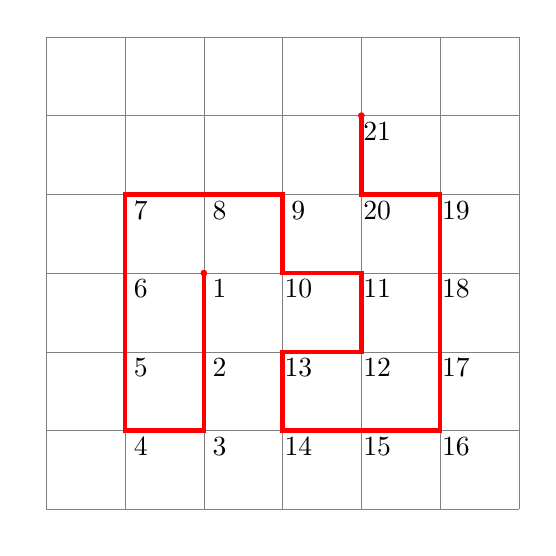
\begin{tikzpicture}[scale=1.00]
% grid
    \foreach \i in {\xMin,...,\xMax} {
        \draw [very thin,gray] (\i,\yMin) -- (\i,\yMax)  node [below] at (\i,\yMin) {};
    }
    \foreach \i in {\yMin,...,\yMax} {
        \draw [very thin,gray] (\xMin,\i) -- (\xMax,\i) node [left] at (\xMin,\i) {};
    }

% start and end of the self avoiding walk
\filldraw[red] (2,3) circle (1pt);
\filldraw[red] (4,5) circle (1pt);

% self avoiding walk
\draw[red, ultra thick] (2,3) -- (2,2) -- (2,1) -- (1,1) -- (1,2) -- (1,3) -- (1,4) -- (2,4) --
(3,4) -- (3,3) -- (4,3) -- (4,2) -- (3,2) -- (3,1) -- (4,1) -- (5,1) -- (5,2) -- (5,3) --
(5,4) -- (4,4) -- (4,5);

% self avoiding walk indexing
\node (A) at (2+\xshift,3+\yshift) {1};
\node (B) at (2+\xshift,2+\yshift) {2};
\node (C) at (2+\xshift,1+\yshift) {3};
\node (D) at (1+\xshift,1+\yshift) {4};
\node (E) at (1+\xshift,2+\yshift) {5};
\node (F) at (1+\xshift,3+\yshift) {6};
\node (G) at (1+\xshift,4+\yshift) {7};
\node (H) at (2+\xshift,4+\yshift) {8};
\node (I) at (3+\xshift,4+\yshift) {9};
\node (J) at (3+\xshift,3+\yshift) {10};
\node (K) at (4+\xshift,3+\yshift) {11};
\node (L) at (4+\xshift,2+\yshift) {12};
\node (M) at (3+\xshift,2+\yshift) {13};
\node (N) at (3+\xshift,1+\yshift) {14};
\node (O) at (4+\xshift,1+\yshift) {15};
\node (P) at (5+\xshift,1+\yshift) {16};
\node (Q) at (5+\xshift,2+\yshift) {17};
\node (R) at (5+\xshift,3+\yshift) {18};
\node (S) at (5+\xshift,4+\yshift) {19};
\node (T) at (4+\xshift,4+\yshift) {20};
\node (U) at (4+\xshift,5+\yshift) {21};



\end{tikzpicture} 